\section{Additional final-candidate results}
Tables~\ref{tab:no_change} and~\ref{tab:weights} retain the complete
no-change comparison and predeclared cost sensitivity. Figure~\ref{fig:prefix}
shows descriptive prefixes of the same fixed policies.
\begin{table*}[t]
\centering\small
\begin{tabular}{lrrrrrr}
\toprule
Method & EM (\%) & F1 (\%) & Utility & Tokens / $S$ item & Pairs & Correct / break \\
\midrule
Closure EVSI (nominee) & 60.430 & 71.646 & 0.560881 & 8683.25 & 6.525 & 62 / 45 \\
EVSI fixed price & 60.430 & 71.646 & 0.560791 & 8701.08 & 6.525 & 62 / 45 \\
EVSI no cost ranking & 60.391 & 71.644 & 0.560400 & 8701.16 & 6.525 & 61 / 45 \\
EVSI old graph cost & 60.430 & 71.646 & 0.560881 & 8683.25 & 6.525 & 62 / 45 \\
Random & 60.508 & 71.732 & 0.561029 & 8809.79 & 8.000 & 64 / 45 \\
Periodic & 60.508 & 71.763 & 0.561496 & 8716.38 & 8.000 & 63 / 44 \\
Uncertainty & 60.469 & 71.685 & 0.560359 & 8865.63 & 8.000 & 62 / 44 \\
Changed first & 60.547 & 71.773 & 0.561855 & 8722.67 & 8.000 & 64 / 44 \\
Stale & 60.430 & 71.646 & 0.563911 & 8077.16 & 0.000 & 64 / 47 \\
Protect changed & 60.430 & 71.646 & 0.563911 & 8077.16 & 0.000 & 64 / 47 \\
Keep (with init.) & 59.766 & 70.968 & 0.556912 & 8148.95 & 0.000 & 0 / 0 \\
Keep (no init.) & 59.766 & 70.968 & 0.563482 & 6834.75 & 0.000 & 0 / 0 \\
Delete changed (no init.) & 60.742 & 71.718 & 0.573606 & 6763.10 & 0.000 & 68 / 43 \\
Delete other (no init.) & 60.312 & 71.543 & 0.569307 & 6763.57 & 0.000 & 61 / 47 \\
Single Qwen & 57.578 & 65.539 & 0.568207 & 1514.93 & 0.000 & 294 / 350 \\
Vote Qwen (3) & 57.891 & 65.895 & 0.556182 & 4544.88 & 0.000 & 300 / 348 \\
Independent 3 + Qwen & 58.984 & 70.520 & 0.556352 & 6698.34 & 0.000 & 191 / 211 \\
\bottomrule
\end{tabular}
\caption{No-change service results. Each method has 512 distinct service questions and 2,560 question--seed observations. Tokens include initialization and feedback; pairs are per episode--seed. Corrections/breakages use the matched keep output. No uncertainty intervals are shown.}
\label{tab:no_change}
\end{table*}

\begin{table*}[t]
\centering\small
\begin{tabular}{lrrrr}
\toprule
Method & $\lambda=0$ & $0.005/1000$ & $0.02/1000$ & $0.05/1000$ \\
\midrule
Closure EVSI (nominee) & 0.605078 & 0.567215 & 0.453627 & 0.226449 \\
EVSI fixed price & 0.605078 & 0.567048 & 0.452957 & 0.224774 \\
EVSI no cost ranking & 0.605078 & 0.567041 & 0.452930 & 0.224708 \\
EVSI old graph cost & 0.608984 & 0.569451 & 0.450852 & 0.213653 \\
Random & 0.605078 & 0.566282 & 0.449894 & 0.217118 \\
Periodic & 0.603516 & 0.566172 & 0.454139 & 0.230074 \\
Uncertainty & 0.605469 & 0.566661 & 0.450237 & 0.217388 \\
Changed first & 0.607812 & 0.567563 & 0.446813 & 0.205314 \\
Stale & 0.605078 & 0.571291 & 0.469928 & 0.267203 \\
Protect changed & 0.616406 & 0.576462 & 0.456630 & 0.216965 \\
Keep (with init.) & 0.606250 & 0.565966 & 0.445116 & 0.203415 \\
Keep (no init.) & 0.606250 & 0.572537 & 0.471400 & 0.269125 \\
Delete changed (no init.) & 0.601172 & 0.575727 & 0.499393 & 0.346725 \\
Delete other (no init.) & 0.617969 & 0.584613 & 0.484547 & 0.284415 \\
Single Qwen & 0.575781 & 0.568207 & 0.545483 & 0.500035 \\
Vote Qwen (3) & 0.578906 & 0.556182 & 0.488009 & 0.351662 \\
Independent 3 + Qwen & 0.589844 & 0.556352 & 0.455877 & 0.254927 \\
\bottomrule
\end{tabular}
\caption{Predeclared descriptive utility sensitivity on the fixed graph-change policies. Policies are not retuned at other weights. The primary weight remains $0.005/1000$.}
\label{tab:weights}
\end{table*}

\begin{figure*}[t]
\centering
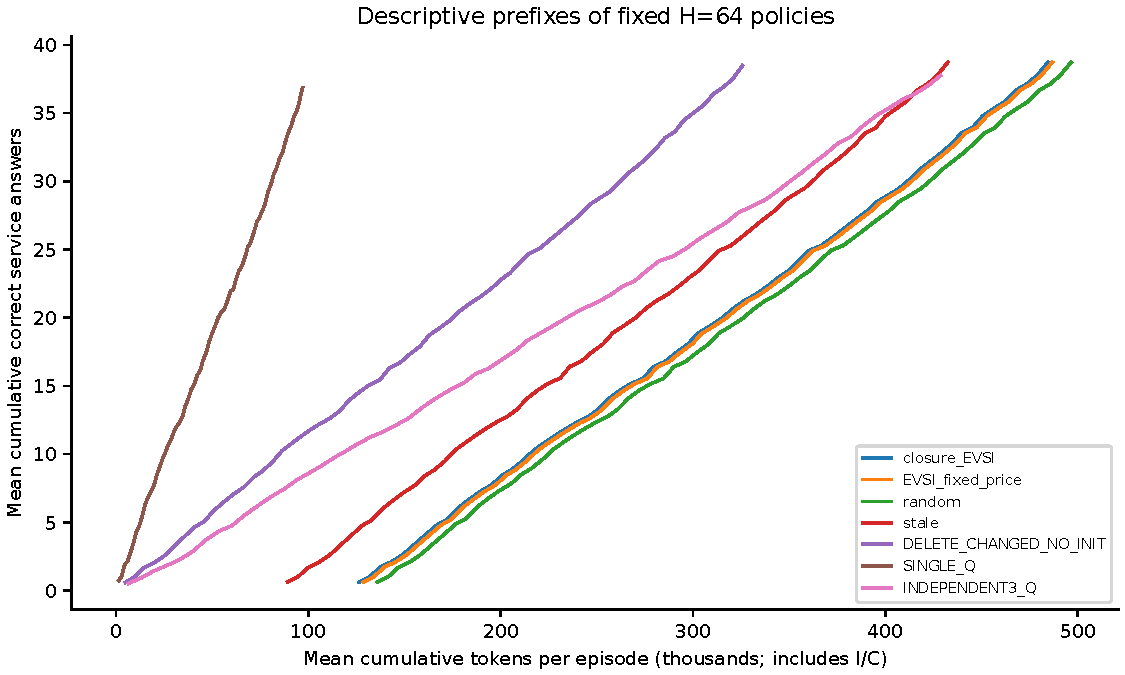
\includegraphics[width=0.95\textwidth]{figures/cumulative_service.pdf}
\caption{Descriptive prefixes of the fixed $H=64$ graph-change policies. The horizontal axis includes all initialization and paid feedback before the first service item; the vertical axis is the mean cumulative number of correct service answers per episode--seed. Policies are not retrained or reoptimized at each prefix. These curves do not establish an optimized equal-spend frontier.}
\label{fig:prefix}
\end{figure*}

\section{Reproduction boundary}
The public aggregate generator reconstructs both 17-method tables,
all five nominee seed points, and the four-weight sensitivity table from
the frozen summary. It reconciles 1,360 episode--seed rows against totals.
The historical generator binds its tables to seven historical source
files by SHA-256. No generator fits a model or resamples data.

The portable experiment bundle passes 36 artificial tests. With authorized
access to private archives, the request auditor reconstructs prompts,
seeds, cache decisions, and stored outputs without model calls. The
independent raw scorer recomputes normalization, exact match, token F1,
and all 3,200 voting decisions; the independent policy auditor rebuilds
paid ledgers and fixed gates. These checks verify limited implementation
properties. They do not regenerate stochastic outputs, supply a new
evaluation cohort, or constitute human review.

The public cost ledger has 11 closed entries: five formal candidates and
six separate engineering qualifications. Cycle GPU residence sums across
workers, including loading and waiting. Historical G2 CUDA-event time
is a separate measurement and is not added to residence or recharged to
this cycle. Unknown human, financial, energy, and complete agent-execution
costs are not imputed as zero. Per-policy logical charges must not be
summed across mutually exclusive policies and interpreted as actual
collection expenditure.

The released code and aggregate artifacts support computational inspection
without exposing raw question-level records. Full private replay requires
the corresponding owner-controlled archive, selection record, approval
files, and pinned model/tokenizer environment. This privacy boundary limits
what an unaffiliated reader can reproduce from public Git alone.
